\documentclass[xcolor=dvipsnames, aspectratio=1610]{beamer}
\usepackage[ngerman]{babel}
\usepackage[T1]{fontenc}
\usepackage[utf8]{inputenc}
\usepackage{lmodern}
\usepackage{stmaryrd}
\usepackage{amsmath}
\usepackage{amsthm}
\usepackage{amssymb}
\usepackage{amsfonts}
\usepackage{enumerate}
\usepackage{colortbl}
\usepackage{tikz}
\usepackage[retainorgcmds]{IEEEtrantools}
\usepackage{mathdots}
\usepackage{tcolorbox}
\usepackage{booktabs}
\usepackage{tabularx}
\tcbuselibrary{theorems}
\usepackage[euler-digits,euler-hat-accent]{eulervm}
\usetikzlibrary{matrix,backgrounds,patterns,arrows,decorations.pathreplacing,shapes,automata}
\usepackage{algorithm}
\usepackage[noend]{algpseudocode}
\usepackage{xifthen}
\usepackage{caption}

\newcommand{\red}[1]{\textcolor{red}{#1}}
\newcommand{\orange}[1]{\textcolor{orange}{#1}}
\newcommand{\green}[1]{\textcolor{markgreen}{#1}}
\newcommand{\textgreen}[1]{\textcolor{textgreen}{#1}}
\newcommand{\gray}[1]{\textcolor{gray}{#1}}

\newcolumntype{R}{>{\centering\raggedleft\arraybackslash}X}
\newcolumntype{L}{>{\centering\raggedright\arraybackslash}X}
\newcolumntype{C}{>{\centering\arraybackslash}X}

\usepackage[firstinits=true,style=ieee-alphabetic,backend=biber]{biblatex}
\addbibresource{knmopr.bib}
\renewcommand*{\bibfont}{\small}

\usefonttheme{professionalfonts} % using non standard fonts for beamer

\setbeamercovered{invisible}

\newcommand{\textsb}[1]{{\fontfamily{cmss}\fontseries{sbc}\fontshape{n}\selectfont #1}}
\newcommand{\tdots}{:}

%ALGORITHMICX
\renewcommand{\algorithmicrequire}{\textcolor{textgreen}{\textbf{Input:}}}
\renewcommand{\algorithmicensure}{\textcolor{textgreen}{\textbf{Output:}}}

% redefine keywords
\algrenewcommand\algorithmicfunction{\textcolor{textgreen}{\textbf{function}}}
\algrenewcommand\algorithmicwhile{\textcolor{textgreen}{\textbf{while}}}
\algrenewcommand\algorithmicfor{\textcolor{textgreen}{\textbf{for}}}
\algrenewcommand\algorithmicif{\textcolor{textgreen}{\textbf{if}}}
\algrenewcommand\algorithmicelse{\textcolor{textgreen}{\textbf{else}}}
\algrenewcommand\algorithmicend{\textcolor{textgreen}{\textbf{end}}}
\algrenewcommand\algorithmicdo{\textcolor{textgreen}{\textbf{do}}}
\algrenewcommand\algorithmicreturn{\textcolor{textgreen}{\textbf{return}}}
\algrenewcommand\algorithmicthen{\textcolor{textgreen}{\textbf{then}}}

% redefine comments
\algrenewcommand{\algorithmiccomment}[1]{{\color{textgreen!80}\textit{\% #1}}}

%COLORBOX
\newtcolorbox{mybox}[1]{
colback=chameleongreen2!30,
colbacktitle=chameleongreen1!50,
coltitle=black,
colframe=textgreen,
boxrule=1pt,
titlerule=0pt,
arc=10pt,
title={\strut\textcolor{textgreen}{\textbf{#1}}}
}
\newtcolorbox{mybluebox}[1]{
colback=chameleongreen4!30,
colbacktitle=chameleongreen4!50,
coltitle=black,
colframe=textblue,
boxrule=1pt,
titlerule=0pt,
arc=10pt,
title={\strut\textcolor{textblue}{\textbf{#1}}}
}

\newcounter{definition}
\resetcounteronoverlays{definition}
\newcommand{\define}{\refstepcounter{definition}\thedefinition}
\newenvironment{defi}{
	\begin{mybox}{Definition \define}
}
{\end{mybox}}

%\newcounter{theorem}
\resetcounteronoverlays{theorem}
\newcommand{\theor}{\refstepcounter{theorem}\thetheorem}
\newenvironment{theo}{
	\begin{mybluebox}{Satz \theor}
}
{\end{mybluebox}}

\newcounter{lemma}
\resetcounteronoverlays{lemma}
\newcommand{\lema}{\refstepcounter{lemma}\thelemma}
\newenvironment{lemm}{
	\begin{mybluebox}{Lemma \lema}
}
{\end{mybluebox}}

\author[Felix Kußmaul]{\Large Felix Kußmaul}
\title[Der KMP-Algorithmus]{\LARGE Der Knuth-Morris-Pratt-Algorithmus}
\subtitle{Einführung und Analyse}
\institute[Uni Siegen]{\normalsize Seminar für Theoretische Informatik\\ Universität Siegen}
\date[29.\ Februar 2016]{\normalsize 29.\ Februar 2016}

\usetheme[pageofpages=/,% String used between the current page and the
                         % total page count.
          titlepagelogo=logo-siegen,% Logo for the first page.
          bullet=triangle,% Use circles instead of squares for bullets.
          titleline=true,% Show a line below the frame title.
          alternativetitlepage=true,% Use the fancy title page.
          ]{Torino}
    
\setbeamercolor{author in head/foot}{bg=chameleongreen3!85}
\setbeamercolor{title in head/foot}{bg=chameleongreen1}
\setbeamercolor{date in head/foot}{bg=chameleongreen4}

\colorlet{markgreen}{chameleongreen3} %chameleongreen3!50!chameleongreen1}
\colorlet{textgreen}{chameleongreen3!70!black}
\colorlet{textblue}{chameleongreen4!70!black}

\setbeamercolor{enumerate item}{fg=textgreen}
%\setbeamercolor{itemize item}{fg=textgreen}

%\setbeamercovered{transparent=80}

\setbeamertemplate{headline}
{
\hbox{%
  \begin{beamercolorbox}[wd=.28\paperwidth,ht=2.7ex,dp=1.2ex,center]{author in head/foot}%
    \usebeamerfont{author in head/foot}\insertshortauthor\ (\insertshortinstitute)
  \end{beamercolorbox}%
  \begin{beamercolorbox}[wd=.44\paperwidth,ht=2.7ex,dp=1.2ex,center]{author in head/foot}%
    \usebeamerfont{title in head/foot}\insertshorttitle:\ \textbf{\insertsection}
  \end{beamercolorbox}%
  \begin{beamercolorbox}[wd=.28\paperwidth,ht=2.7ex,dp=1.2ex,center]{author in head/foot}%
    \usebeamerfont{date in head/foot}\insertshortdate
  \end{beamercolorbox}}
  \vskip0pt%
}

\DeclareMathAlphabet{\mathcal}{OMS}{cmsy}{m}{n}

\tikzset{
  invisible/.style={opacity=0},
  visible on/.style={alt={#1{}{invisible}}},
  alt/.code args={<#1>#2#3}{%
    \alt<#1>{\pgfkeysalso{#2}}{\pgfkeysalso{#3}} % \pgfkeysalso doesn't change the path
  },
}

\newcommand{\printSectionYes}{\AtBeginSubsection[]
{
 \begin{frame}{Agenda}
 \tableofcontents[sectionstyle=show/shaded,
 					subsectionstyle=show/shaded/hide]
 \end{frame}
}}

\tikzset{onslide/.code args={<#1>#2}{%
  \only<#1>{\pgfkeysalso{#2}}%
}}

\setbeamertemplate{section in toc shaded}[default][50]

\makeatletter
\patchcmd{\beamer@sectionintoc}{\vskip1.5em}{\vskip0.5em}{}{}
\makeatother
 
\begin{document}

\frame[t,plain,label=titel]{
	\titlepage
}

\begin{frame}{Agenda}
       \tableofcontents[ 
  		currentsubsection, 
  		hideothersubsections, 
   	 	sectionstyle=show, 
   	 ] 
\end{frame}

\section{Einleitung}

\printSectionYes

\begin{frame}[<+->]{Grundbegriffe}
\begin{defi}
Wir definieren wie üblich:
\begin{enumerate}[(i)]
\item eine nichtleere, endliche Menge von \textit{Zeichen} als \textit{Alphabet} $\Sigma$
\item eine endliche Folge von Zeichen $v=a_1\cdots a_n$ als \textit{Wort} über $\Sigma$, wobei $n\geq 0$ und $a_i\in\Sigma$ mit $i=1,\dots,n$
\item $\Sigma^*$ als die \textit{Kleene'sche Hülle} von $\Sigma$ (Menge aller Wörter über $\Sigma$)
\item $v[i]=a_i$ als das \textit{$i$-te Zeichen} von $v=a_1\cdots a_n$ \hfill($i=1,\dots,n$, $n\geq 0$)
\end{enumerate}
\end{defi}
\end{frame}

\begin{frame}[<+->]{Grundbegriffe}
\begin{mybox}{Definition \thedefinition\ (Fortsetzung).}
\begin{enumerate}[(i)]\setcounter{enumi}{4}
\item $\vert v\vert=n$ als die \textit{Länge} von $v=a_1\cdots a_n$\hfill($n\geq 0$)
\item die \textit{Konkatenation} zweier Wörter $v=a_1\cdots a_n$ und $w=b_1\cdots b_m$: $v\circ w=a_1\cdots a_nb_1\cdots b_m$ \hfill($n,m\geq 0$)
\item $\varepsilon$ als das \textit{leere Wort} mit $v\circ\varepsilon = v$ und $\varepsilon\circ v=v$\hfill($v\in\Sigma^*$)
\item $v^n$ als die \textit{$n$-te Potenz} von $v$ mit $v^n=v\circ v^{n-1}$ und $v^0 =\varepsilon$
\end{enumerate}
\end{mybox}
\end{frame}

\begin{frame}[<+->]{Grundbegriffe}
\begin{defi}
Seien $v,x$ Wörter über $\Sigma$.
\begin{enumerate}[(i)]
\item $v$ heißt \textit{Präfix} von $x$, falls $u\in\Sigma^*$ ex.\ mit $x=vu$.
\item $v$ heißt \textit{Suffix} von $x$, falls $u\in\Sigma^*$ ex.\ mit $x=uv$.
\item $v$ heißt \textit{Teilwort} von $x$, falls $u,w\in\Sigma^*$ ex.\ mit $x=uvw$.
\item Präfix, Suffix oder Teilwort $v$ von $x$ heißt \textit{echt}, falls $v\neq x$.
\end{enumerate}
\end{defi}
\end{frame}

\begin{frame}[<+->]{Grundbegriffe Komplexität}
\begin{defi}
Für eine gegebene Funktion $g(n)$ definieren wir die Mengen
\begin{enumerate}[(i)]
\item $\mathcal{O}\big(g(n)\big)=\big\{f(n)\;\big\vert\;\exists c,n_0\;\forall n\geq n_0 :\; 0\leq f(n)\leq cg(n)\big\}$
\item $\Omega\big(g(n)\big)=\big\{f(n)\;\big\vert\;\exists c,n_0\;\forall n\geq n_0 :\; 0\leq cg(n)\leq f(n)\big\}$
\item $\Theta\big(g(n)\big)=\big\{f(n)\;\big\vert\;\exists c_1,c_2,n_0\;\forall n\geq n_0 :\; 0\leq c_1g(n)\leq f(n)\leq c_2g(n)\big\}$
\end{enumerate}
\end{defi}\medskip
\onslide<4>{\textit{Ohne Beweis:} Für zwei Funktionen $f(n),\,g(n)$ gilt $f(n)\in\Theta\big(g(n)\big)$ genau dann, wenn $f(n)\in\mathcal{O}\big(g(n)\big)$ und $f(n)\in\Omega\big(g(n)\big)$.\qed}
\end{frame}

\begin{frame}[<+->]{Konventionen}
Sei $\Sigma$ ein Alphabet. Wir schreiben\bigskip

\begin{itemize}
\item $\Sigma^+$ für $\Sigma^*\setminus \{\varepsilon\}$, also die Menge aller \textit{nichtleeren} Wörter über $\Sigma$
\item Kleinbuchstaben vom Alphabetanfang ($a,b,c,\dots$) für Zeichen in $\Sigma$
\item Kleinbuchstaben vom Alphabetende ($u, v, w,\dots$) für Wörter über $\Sigma$
\item $v\circ w$ kurz als $vw$
\item $u[1] u[2] \cdots u[n]$ kurz als $u[1 \tdots n]$\hfill ($n\geq 0$)
%\item Beschränkung auf Binärstrings, also $\Sigma = \{0,1\}$

\end{itemize}
\end{frame}

\section{Motivation}
\subsection{Das String-Matching-Problem}
%\begin{frame}{Das String-Matching-Problem}
%\begin{mybox}{String-Matching-Problem}
%Seien $p,w\in\Sigma^+$ Wörter mit $\vert p\vert \leq \vert w\vert$. Existieren zwei Wörter $u,v$, sodass \[w=upv\quad \text{?}\]\pause
%Mit anderen Worten: Ist $p$ ein Teilwort von $w$?
%\end{mybox}\bigskip
%
%Konkret suchen wir nach der Position $\vert u\vert +1$ von $p$ in $w$.
%\end{frame}

\begin{frame}[<+->]{Das String-Matching-Problem}
\begin{defi}
Seien $p,t\in\Sigma^+$ Wörter mit $\vert p\vert \leq \vert t\vert$ und sei $s\in\mathbb{N}$.\medskip

Wir schreiben, dass Muster $p$ \emph{mit Shift $s$} in Text $t$ \emph{vorkommt}, wenn
\begin{IEEEeqnarray}{C"l}
t[s+i] = p[i]&\text{für }1\leq i\leq \vert p\vert\text{ und}\\
0\leq s\leq \vert t\vert-\vert p\vert
\end{IEEEeqnarray}
In diesem Fall heißt $s$ \emph{gültig}, ansonsten \emph{ungültig}.
\end{defi}
\end{frame}

\begin{frame}{Das String-Matching-Problem}
\begin{mybox}{String-Matching-Problem}
Das \emph{String-Matching-Problem} ist das Problem, alle gültigen Shifts zu finden, mit denen $p$ in $w$ vorkommt.
\end{mybox}
\end{frame}

\subsection{Naiver Suchalgorithmus}
\begin{frame}{Naiver Suchalgorithmus}
\textbf{Informal:}

\begin{enumerate}[1.]
\item<2-> Baue aus der Suchmaske ein Fenster und schiebe es an den Anfang.
\item<3-> Vergleiche jedes Zeichen im Fenster mit Textzeichen darunter:
\begin{itemize}
\item Falls ungleich, schiebe Fenster um eins weiter.
\item Falls Ende des Fensters erreicht: \textbf{Fund}.
\end{itemize}
\item<8> Halt, falls \texttt{EOF} erkannt.
\end{enumerate}
FARBEN ÜBERARBEITEN
\begin{center}
\begin{tikzpicture}[thick, scale=0.9, anchor=base ]
\node (st) at (-.5,-0.5) {\small Suchtext};
\node[visible on=<2->](sm) at (-.5,-1.7) {\small Suchmaske};

\foreach \x/\y/\z in {1/0/3,2/1/0,3/1/5,4/0/0,5/0/0,6/1/0,7/0/0} {
	\draw[fill=chameleongreen2!40] (\x,-.85) rectangle (\x+1,0.15);
	\ifthenelse{1=\x \OR \x=3}{
    	\node[onslide=<\z>{text=red}] at (\x+.5,-0.5) {\Large $\texttt{\y}$};
    }{\node at (\x+.5,-0.5) {\Large $\texttt{\y}$};}
}

\draw<2-3>[color= chameleongreen4] (0.95,-.9) rectangle (4.05,.2);
\node(p1)[visible on=<2>]  at (2.5,0.40) {\footnotesize\textcolor{chameleongreen4}{Fenster}};
\draw<4-5>[color= chameleongreen4] (1.95,-.9) rectangle (5.05,.2);
\node(p2)[visible on=<4-5>] at (3.5,0.40) {};
\draw<6-8>[color= chameleongreen4] (2.95,-.9) rectangle (6.05,.2);
\node(p3)[visible on=<6-8>] at (4.5,0.40) {};

\node[visible on=<3>, right of=p1] {\textcolor{chameleongreen4}{$\to$}};
\node[visible on=<5>, right of=p2] {\textcolor{chameleongreen4}{$\to$}};

\draw[visible on=<1>, color=white] (1,-2.05) rectangle (2,-1.2);

\foreach \x/\y/\z in {2/1/3,3/0/5,4/0/0} {
	\draw<2-3>(\x-1,-2.05) rectangle (\x,-1.05);
	\ifthenelse{\x=2}{
		\node<2-3>[onslide=<\z>{text=red}] at (\x-.5,-1.7) {\Large $\texttt{\y}$};
	}{\node<2-3> at (\x-.5,-1.7) {\Large \texttt{\y}};}
    \draw<4-5> (\x,-2.05) rectangle (\x+1,-1.05);
    \ifthenelse{\x=3}{
		\node<4-5>[onslide=<\z>{text=red}] at (\x+.5,-1.7) {\Large $\texttt{\y}$};
	}{\node<4-5> at (\x+.5,-1.7) {\Large \texttt{\y}};}
    \draw<6-8> (\x+1,-2.05) rectangle (\x+2,-1.05);
    \node<6-8> at (\x+1.5,-1.7) {\Large \texttt{\y}};
}

\node<4-5> at (2.5,-1.7) {\textcolor{markgreen}{\Large \texttt{1}}};
\node<6-8> at (3.5,-1.7) {\textcolor{markgreen}{\Large \texttt{1}}};
\node<7-8> at (4.5,-1.7) {\textcolor{markgreen}{\Large \texttt{0}}};
\node<8> at (5.5,-1.7) {\textcolor{markgreen}{\Large \texttt{0}}};

\node[visible on=<8>, right of=p3]  {\textcolor{markgreen}{\quad\Large $\checkmark$\normalsize $~s=2$}};
\end{tikzpicture}
\end{center}
\end{frame}

\begin{frame}[label=naive]{Naiver Suchalgorithmus}
\begin{mybox}{Naiver Suchalgorithmus \cites{cormenalgorithms2009}{berman2005algorithms}}
\begin{algorithmic}[lines]
\Require{Suchtext $t=a_1\cdots a_n$, Muster $p=b_1\cdots b_m$}
\Ensure{Liste gültiger Shifts $s$ von $p$ in $t$}\\\\

\centering
\parbox[l]{8cm}{
\For{$s=0$ \textcolor{textgreen}{\textbf{to}} $n-m$}
	\If {$t\big[(s+1)\tdots (s+m)\big] ==\: p[1 \tdots m]$}
		\State \textgreen{\textbf{add}} $s$ \textgreen{\textbf{to}} results
	\EndIf
\EndFor

\Return{results}
}
\end{algorithmic}
\end{mybox}
\textit{Obacht:} In Zeile 2 versteckt sich eine lineare Suche!
\end{frame}

\begin{frame}{Naiver Suchalgorithmus}
Die Schritte zusammengefasst:\bigskip

\begin{minipage}{.9\textwidth}
\begin{table}\setlength\extrarowheight{.3em}
\begin{tabularx}{8cm}{CCC@{\hskip 2em}ccccccc}
\toprule
 &&	& 1 				& 2 				& 3 				& 4 				& 5 				& 6 				& 7 \\
$s$&$j$	& $s+j$			&\texttt{0}			&\texttt{1}			&\texttt{1}			&\texttt{0}			&\texttt{0}			&\texttt{1}			&\texttt{0}\\
\midrule
 0 			& 1 			& 1 			&\red{\texttt{1}}	&\gray{\texttt{0}}	&\gray{\texttt{0}}\\
 1 			& 2 			& 3 			&					&\texttt{1}			&\red{\texttt{0}}	&\gray{\texttt{0}}\\
\green{ 2 }	& 3 			& 5 			&					&					&\texttt{1}			&\texttt{0}			&\texttt{0}\\
 3 			& 1 			& 4 			&					&					&					&\red{\texttt{1}}	&\gray{\texttt{0}}	&\gray{\texttt{0}}\\
 4 			& 1 			& 5 			&					&					&					&					&\red{\texttt{1}}	&\gray{\texttt{0}}	&\gray{\texttt{0}}\\
\bottomrule
\end{tabularx}
\caption{Naiver Algorithmus, Beispiel}
\end{table}
\end{minipage}
\hspace{-4em}
\begin{minipage}{0.05\textwidth}
\tiny\vspace{-4em}
\begin{tabular}{cl}
\cellcolor{markgreen}~~& gültige Shifts\\\\[-.5em]
\cellcolor{red}~~& Mismatches\\\\[-.5em]
\cellcolor{lightgray}~~& ausgelassene Vergleiche
\end{tabular}
\end{minipage}
\end{frame}

\begin{frame}[<+->]{Komplexitätsmessung}
Zur Komplexitätsmessung betrachten wir die \textbf{Anzahl der Vergleiche} von Zeichen.\bigskip

\begin{itemize}
\item Im Pseudocode: Prüfung von \emph{gleichlangen} Strings in einer Zeile\bigskip
\item Der zeichenweise Vergleich von zwei Strings $v,w$ bis zu einem Mismatch kostet \[\Theta\big(\vert u\vert +1\big)\] bei Mismatch an Stelle $\vert u\vert +1$, wenn gilt: $u$ ist Präfix von $v$ und  $u$ ist Präfix von $w$.
\end{itemize}
\end{frame}

\begin{frame}{Naiver Suchalgorithmus: Analyse}
Der naive Algorithmus hat eine Laufzeit von \[V=\underbrace{(n-m+1)}_{\text{Schleife außen}}\cdot \underbrace{m}_{\text{innen}}\in\mathcal{O}(nm)\]\medskip\pause

\textbf{Best Case:}\medskip

Jeder Versuch wird bereits beim ersten Zeichen abgebrochen:
\[V=n-m+1\in\Theta(n)\]
\end{frame}

\begin{frame}{Naiver Suchalgorithmus: Analyse}
\textbf{Worst Case:}\medskip

Das Muster wird immer bis zum Ende gescannt und dann abgebrochen. Dann gilt:
\[V=(n-m+1)\cdot m\in\Theta(nm)\]\smallskip\pause

\textit{Klassisches Beispiel:}\smallskip

Suche Muster $p=a^{m-1}b$ in Text $t=a^n$. So z.\,B.:
\begin{IEEEeqnarray*}{rCl}
t&=&\texttt{00000000000000}\\
p&=&\texttt{001}
\end{IEEEeqnarray*}
mit $a=\texttt{0}$, $b=\texttt{1}$.
\end{frame}

\begin{frame}<1-5>[label=ani]
\frametitle<1-5>{Naiver Suchalgorithmus: Auswertung}
\frametitle<6->{KMP-Algorithmus}
\begin{large}\textbf{Einige Fragen:}\end{large}\medskip\pause
\begin{enumerate}[(1)]
\item Was macht die Ineffizienz beim naiven Algorithmus aus? \smallskip\pause

$\Rightarrow$ Überflüssige Vergleiche!\pause\smallskip
\item Welche Vergleiche sind überflüssig?

\smallskip\pause

$\Rightarrow$ Mehrfache Vergleiche, aber wie findet man die heraus?\pause

\begin{enumerate}[(a)]
\item Bereits gescannte Zeichen, die kein Präfix des Musters sind\pause
\item Ein erkanntes Präfix, das in der inneren Schleife übersprungen werden kann\pause
\end{enumerate}

\item Woher wissen wir \textbf{sicher} für jede Position im Muster, wie viele Zeichen wir überspringen dürfen?
\end{enumerate}
\end{frame}

\section{Knuth-Morris-Pratt-Algorithmus}

\subsection{Geschichte}

\begin{frame}{Geschichte}
\begin{minipage}{0.3\textwidth}
\begin{figure}
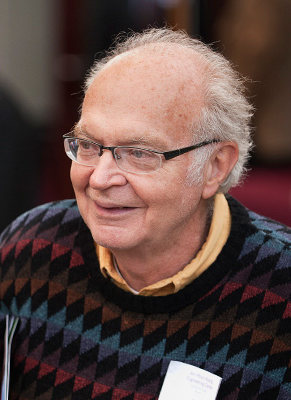
\includegraphics[width=.8\textwidth]{knuth}
\caption{Donald E.\ Knuth}
\end{figure}
\end{minipage}
\hfill
\begin{minipage}{0.3\textwidth}
\begin{figure}
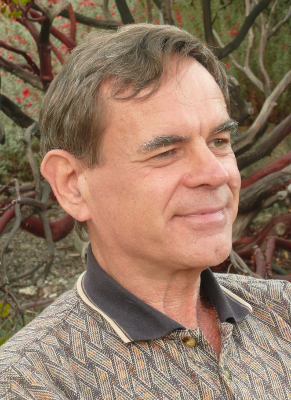
\includegraphics[width=0.8\textwidth]{pratt}
\caption{Vaughan Pratt}
\end{figure}
\end{minipage}
\hfill
\begin{minipage}{0.3\textwidth}
\begin{figure}
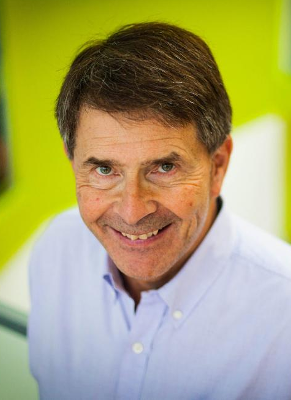
\includegraphics[width=.8\textwidth]{morris}
\caption{James H.\ Morris}
\end{figure}
\end{minipage}
\end{frame}

\subsection{Einführung}

\begin{frame}{Einführungsbeispiel}
\begin{center}\vspace*{-1em}
\begin{tikzpicture}[visible on=<1-4>,thick, scale=1, anchor=base ]

\foreach \x/\y in {1/a,2/b,3/c,4/d,5/a,6/b,7/c,8/a,9/b,10/c,11/a,12/b,13/d} {
	\draw[fill=chameleongreen2!50] (\x,-.85) rectangle (\x+1,0.15);
    \node at (\x+.5,-0.5) {\Large \texttt{\y}};
    \node at (\x+.5,0.3) {\tiny \texttt{\x}};
}

%\node<1> at (1,-3.3) {$s=0$};
\node<2> at (2.5,-2) {$s=3$};
\node<3> at (3,-2) {$s=4$};
\node<4> at (4.5,-2) {$s=7$};

\draw<2>[|->] (1,-1.55) -- (4,-1.55);
\draw<3>[|->] (1,-1.55) -- (5,-1.55);
\draw<4>[|->] (1,-1.55) -- (8,-1.55);

\node at (0.3,-2.4) {\tiny $j$};
\node<1-4> at (0.3,-0.5) {\small $t$};
\node<1-4> at (0.3,-1.7) {\small $p$};

\draw<1>[color= chameleongreen4] (0.95,-.9) rectangle (7.05,.2);
\draw<2>[color= chameleongreen4] (3.95,-.9) rectangle (10.05,.2);
\draw<3>[color= chameleongreen4] (4.95,-.9) rectangle (11.05,.2);
\draw<4>[color= chameleongreen4](7.95,-.9) rectangle (14.05,.2);

\node<-3> at 	(10.32,-2.9) {\textcolor{white}{ \rotatebox[origin=c]{270}{\Huge $\Lsh$}}};
%anti-slip
%\draw<2-4>[color=white] (0.95,0) -- (0.95,-0.05);
%\draw[color=white] (14.95,0) -- (14.95,-0.05);
%\draw[visible on=<1-5>, color=white] (1,-2.05) rectangle (2,-1.2);

\foreach \x/\y in {1/a,2/b,3/c,4/a,5/b,6/d} {
	\draw<1> 	(\x,-2.05) rectangle (\x+1,-1.05);
    \node<1> at (\x+.5,-1.7) {\Large \texttt{\y}};
    \node<1> at (\x+.5,-2.4) {\tiny \texttt{\x}};
    \draw<2> 	(\x+3,-2.05) rectangle (\x+4,-1.05);
    \node<2> at (\x+3.5,-1.7) {\Large \texttt{\y}};
    \node<2> at (\x+3.5,-2.4) {\tiny \texttt{\x}};
    \draw<3> 	(\x+4,-2.05) rectangle (\x+5,-1.05);
    \node<3> at (\x+4.5,-1.7) {\Large \texttt{\y}};
    \node<3> at (\x+4.5,-2.4) {\tiny \texttt{\x}};
    \draw<4> 	(\x+7,-2.05) rectangle (\x+8,-1.05);
    \node<4>at (\x+7.5,-1.7) {\Large \texttt{\y}};
    \node<4>at (\x+7.5,-2.4) {\tiny \texttt{\x}};
}

%coloured s and j's
%\node<1> at (1.5,0.3) {\tiny \textcolor{orange}{\texttt{1}}};
%\node<2> at (4.5,0.3) {\tiny \textcolor{orange}{\texttt{4}}};
%\node<3> at (5.5,0.3) {\tiny \textcolor{orange}{\texttt{5}}};
%\node<4> at (8.5,0.3) {\tiny \textcolor{orange}{\texttt{8}}};
\node<1> at (4.5,-2.4) {\tiny \textcolor{orange}{\texttt{4}}};
\node<2> at (4.5,-2.4) {\tiny \textcolor{orange}{\texttt{1}}};
\node<3> at (10.5,-2.4) {\tiny \textcolor{orange}{\texttt{6}}};
\node<4> at (13.5,-2.4) {\tiny \textcolor{orange}{\texttt{6}}};

\node<1> at 	(1.5,-1.7) {\textcolor{markgreen}{\Large \texttt{a}}};
\node<1> at 	(2.5,-1.7) {\textcolor{markgreen}{\Large \texttt{b}}};
\node<1> at 	(3.5,-1.7) {\textcolor{markgreen}{\Large \texttt{c}}};
\node<1> at 	(4.5,-0.5) {\textcolor{red}{\Large \texttt{d}}};
\node<1> at 	(4.5,-1.7) {\textcolor{red}{\Large \texttt{a}}};

\node<2> at 	(4.5,-0.5) {\textcolor{red}{\Large \texttt{d}}};
\node<2> at 	(4.5,-1.7) {\textcolor{red}{\Large \texttt{a}}};

\node<3> at 	(5.5,-1.7) {\textcolor{markgreen}{\Large \texttt{a}}};
\node<3> at 	(6.5,-1.7) {\textcolor{markgreen}{\Large \texttt{b}}};
\node<3> at 	(7.5,-1.7) {\textcolor{markgreen}{\Large \texttt{c}}};
\node<3> at 	(8.5,-1.7) {\textcolor{markgreen}{\Large \texttt{a}}};
\node<3> at 	(9.5,-1.7) {\textcolor{markgreen}{\Large \texttt{b}}};
\node<3> at 	(10.5,-0.5) {\textcolor{red}{\Large \texttt{c}}};
\node<3> at 	(10.5,-1.7) {\textcolor{red}{\Large \texttt{d}}};

\node<4> at 	(10.32,-2.9) {\textcolor{orange}{ \rotatebox[origin=c]{270}{\Huge $\Lsh$}}};
\node<4> at 	(10.5,-1.7) {\textcolor{markgreen}{\Large \texttt{c}}};
\node<4> at 	(11.5,-1.7) {\textcolor{markgreen}{\Large \texttt{a}}};
\node<4> at 	(12.5,-1.7) {\textcolor{markgreen}{\Large \texttt{b}}};
\node<4> at 	(13.5,-1.7) {\textcolor{markgreen}{\Large \texttt{d}}};

\node[visible on=<4>] at (13.9,.3) {\textcolor{markgreen}{\Large $\checkmark$}};
\end{tikzpicture}
\end{center}
\end{frame}

\begin{frame}{Einführungsbeispiel}
\begin{table}\setlength\extrarowheight{.3em}
\begin{tabularx}{.8\textwidth}{CC@{\hskip 2em}ccccccccccccc}
\toprule
& & 1 & 2 & 3 & 4 & 5 & 6 & 7 & 8 & 9 & 10 & 11 & 12&13 \\
$s$ & $j$ &a&b&c&d&a&b&c&a&b&c&a&b&d\\
\midrule
0 & 4 & a & b & c & \red{a} & \gray{b} & \gray{d} &&&&&&&\\ 
3 & 1 &&&& \red{a} & \gray{b} & \gray{c} & \gray{a} & \gray{b} & \gray{d} &&&&\\ 
4 & 6 &&&&& a & b & c & a & b & \red{d} &&&\\ 
\green{7} & 7 &&&&&&&& \gray{a} & \gray{b} & c & a & b & d \\
\bottomrule
\end{tabularx}
\caption{KMP-Algorithmus, Beispiel}
\end{table}
\end{frame}

\begin{frame}{Einführung}
\textbf{Beobachtung:} Finden wir ein \textit{Präfix $u$ des Musters $p$} im erfolgreich gescannten Teil $v$ wieder, können wir dieses als \glqq Fallback-Position\grqq\ nutzen.\bigskip\medskip

\begin{center}
\resizebox {0.9\textwidth} {!} {
\begin{tikzpicture}[thick, anchor=base ]

% t
%\draw[fill=white] (13,2) rectangle (16,3);
\draw[fill=chameleongreen2!35] (0,2) rectangle (12,3);
\draw (-1,2) -- (0,2);
\draw (-1,3) -- (0,3);
\node at (-.5,2.5) {\dots};
\draw (13,2) -- (14,2);
\draw (13,3) -- (14,3);
\node at (13.5,2.5) {\dots};
\draw (13,1) -- (14,1);
\draw (13,0) -- (14,0);
\node at (13.5,0.5) {\dots};
\draw[fill=red!40] (12,2) rectangle (13,3);
\node at (12.55,2.35) {\LARGE $\lightning$};
\draw[dashed] (12,1) -- (12,2);
\draw[dashed] (0,1) -- (0,2);
\draw[dashed] (13,1) -- (13,2);
\node at (-2,2.35) {\LARGE $t$};

\draw[->] (-.7,0.5) -- (0,.5);
\draw[dotted] (-1,0.5) -- (-0.7,.5);
\node at (-.5,0) {\large $s$};

% p
\draw[fill=chameleongreen2] (0,0) rectangle (13,1);
%\draw[fill=white] (13,0) rectangle (16,1);
\draw[fill=chameleongreen2!35] (3,0) rectangle (9,1);
\draw[fill=red!40] (12,0) rectangle (13,1);
\node at (1.5,0.35) {\Large $u$};\node at (10.5,0.35) {\Large $u$};
\node at (12.55,0.35) {\LARGE $\lightning$};
\node at (-2,0.35) {\LARGE $p$};
\node (da) at (12.5,-0.35) {\Large $\uparrow$};
\node[below of=da, node distance=1.5em] {\Large $j+1$};

\node at (6,2.35) {\Large $v$};

\draw [line width=1pt,decorate,decoration={brace,amplitude=10pt,mirror}](0,0) -- (12,0) node[midway,yshift=-2.5em] {\Large $v=p[1\tdots j]$};
\end{tikzpicture}}
\end{center}
\end{frame}

\begin{frame}{Einführung}
\textbf{Idee:}\medskip

Wir erstellen im Vorfeld eine \textit{Tabelle} aus dem Muster, in der wir zur Laufzeit nur nachschlagen müssen.\medskip

Sie verrät uns, um wie viele Schritte das Muster bei einem Mismatch geschoben werden muss.
\end{frame}

\begin{frame}{KMP-Algorithmus}
Der KMP-Algorithmus wird folglich in zwei Phasen aufgeteilt:\bigskip

\begin{enumerate}[1.]
\item \textit{Vorlauf:} Analyse des Suchmusters und Erstellen der Nachschlagetabelle
\item \textit{Suche:} Suche im Text mithilfe der Tabelle
\end{enumerate}
\end{frame}

\subsection{Vorlaufphase}

\begin{frame}{Präfixfunktion}
\begin{defi}
Seien $u,x$ Wörter über $\Sigma$ mit $\vert u\vert <\vert x\vert$. Wir nennen $u$ \textit{Rand} von $x$, falls $v,w\in\Sigma^+$ ex.\ mit \[x=uv=wu\]
\end{defi}
\pause\bigskip
Mit anderen Worten:\smallskip

Ein Rand ist sowohl \emph{echtes Präfix}, als auch \emph{echtes Suffix} eines Wortes.
\end{frame}

\begin{frame}{Präfixfunktion}
\textbf{Beispiel:}\bigskip

Sei $p=\texttt{011110110}$. Wie lautet die Menge der Ränder von $p$?\pause

\[\{\varepsilon,\texttt{0}\}\]
\end{frame}

\begin{frame}{Präfixfunktion}
\textbf{Noch ein Beispiel:}\bigskip

Sei $p=\texttt{0101010101}$. Wie lautet die Menge der Ränder von $p$?\pause

\[\{\varepsilon,\texttt{01},\texttt{0101},\texttt{010101},\texttt{01010101}\}\]
\end{frame}

\begin{frame}{Präfixfunktion}
\begin{center}
\resizebox {0.8\textwidth} {!} {
\begin{tikzpicture}[thick, anchor=base ]
% t
\draw[visible on=<1-2>,fill=chameleongreen2!35] (1,2) rectangle (12,3);
\draw<2>[fill=chameleongreen2] (7,2) rectangle (12,3);
%\draw[fill=chameleongreen2] (11,2) rectangle (12,3);

\node[visible on=<1-2>] at (1.5,2.35) {$s+1$};
\node<2> at (7.5,2.35) {\small $s'+1$};
\node<1> at (11.5,2.35) {$s+j$};
\node<2> at (11.5,2.35) {\small $s'+k$};
\draw[visible on=<1-2>] (-1,2) -- (1,2);
\draw[visible on=<1-2>] (-1,3) -- (1,3);
\node[visible on=<1-2>] at (0,2.5) {\dots};
\draw[visible on=<1-2>] (13,2) -- (14,2);
\draw[visible on=<1-2>] (13,3) -- (14,3);
\node[visible on=<1-2>] at (13.5,2.5) {\dots};

\draw[visible on=<1-2>,fill=red!40] (12,2) rectangle (13,3);
\node[visible on=<1-2>] at (12.55,2.35) {\LARGE $\lightning$};
\node[visible on=<1-2>] at (-2,2.35) {\LARGE $t$};

% p
\draw[fill=chameleongreen2!35] (1,0) rectangle (12,1);
\draw<3->[fill=chameleongreen2] (7,0) rectangle (12,1);
\draw<4>[fill=chameleongreen2] (1,0) rectangle (6,1);
%\draw (1,0) rectangle (2,1);
%\draw[fill=chameleongreen2] (11,0) rectangle (12,1);
\draw[fill=red!40] (12,0) rectangle (13,1);
\node at (1.5,0.35) {\Large $1$};\node at (11.5,0.35) {\Large $j$};
\node at (12.55,0.35) {\LARGE $\lightning$};
\node at (-2,0.35) {\LARGE $p$};

\node<4> at (5.5,0.35) {\Large $k$};
%\node (da) at (12.5,-0.35) {\Large $\uparrow$};
%\node[below of=da, node distance=1.5em] {\Large $j+1$};

\draw (13,1) -- (14,1);
\draw (13,0) -- (14,0);
\node at (13.5,0.5) {\dots};

\draw[->] (-.7,0.5) -- (1,.5);
\draw[dotted] (-1,0.5) -- (-0.7,.5);
\node at (0,0) {\large $s$};

%p'
\node[visible on=<2->] at (-2,-1.65) {\LARGE $p'$};
%\draw[visible on=<2>,fill=chameleongreen2!35] (7,-1) rectangle (13,-2);
\draw[visible on=<2->,fill=chameleongreen2] (7,-1) rectangle (13,-2);

\node[visible on=<2->] at (7.5,-1.65) {\Large $1$};
\node[visible on=<2->] at (11.5,-1.65) {\Large $k$};
\draw[visible on=<2->] (13,-1) -- (14,-1);
\draw[visible on=<2->] (13,-2) -- (14,-2);
\node[visible on=<2->] at (13.5,-1.5) {\dots};
\draw[visible on=<2->,fill=orange!40] (12,-1) rectangle (13,-2);
\node[visible on=<2->]  at (12.55,-1.65) {\Large $?$};
\draw[visible on=<2->,dashed] (7,-1) -- (7,2);
\draw[visible on=<2->,dashed] (8,-2) -- (8,3);
\draw[visible on=<2->,dashed] (11,0) -- (11,-2);
\draw[visible on=<2->,dashed] (12,0) -- (12,-1);

\draw [dashed] (12,0) -- (12,3);
\draw [visible on=<1-2>,dashed] (13,1) -- (13,2);
\draw [visible on=<1-2>,dashed] (1,1) -- (1,2);
\draw [dashed] (2,0) -- (2,3);
\draw [dashed] (11,0) -- (11,3);

\draw [visible on=<4>,dashed] (5,0) -- (5,1);

\draw [visible on=<2->,->] (-.7,-1.5) -- (7,-1.5);
\draw [visible on=<2->,dotted] (-1,-1.5) -- (-0.7,-1.5);
\node [visible on=<2->] at (3,-2) {\large $s'$};

\fill[visible on=<3->,fill=white] (1,1.01) rectangle (13,3);
\end{tikzpicture}}
\end{center}\medskip

Ang., $p[1\tdots j] == t\big[(s+1)\tdots(s+j)\big]$.\only<1>{\bigskip\bigskip\bigskip\bigskip} \only<2-3>{Was ist das kleinste $s'>s$, sodass für ein $k<j$:\[p[1\tdots k] == t\big[(s'+1)\tdots(s'+k)\big]\] gilt, mit $s'+k=s+j$?}
\only<4>{Was ist das größte $k<j$, sodass:\[p[1\tdots k] \text{ ist Rand von } p[1\tdots j]\] gilt, mit $s'=s+(j-k)$ und $s'$ als nächstem Shift-Kandidaten?}
\end{frame}

\begin{frame}{Präfixfunktion}
Wir suchen also die Länge $k$ des größten Randes von $p[1\tdots j]$ für alle $j$ mit $1\leq j\leq\vert p\vert$.\bigskip\pause

Als Hilfsmittel wollen wir eine Funktion $\pi_p$ definieren, sodass $\pi_p(j)=k$.\bigskip\pause

\textit{Mismatch bei $j$:} Wir dürfen $j-\pi_p(j)$ Schritte weiterschieben (relativ zu $s$)!
\end{frame}

\begin{frame}{Präfixfunktion}
\begin{defi}
Sei $p$ ein Wort über $\Sigma$ mit $\vert p\vert=m$ und sei $j\geq 1$. Die \emph{Präfixfunktion $\pi_p$ für das Muster $p$} ist definiert durch \[\pi_p\colon\{1,2,\dots,m\}\to\{0,1,\dots,m-1\}\] mit
\[\pi_p(j)=\mathrm{max}\Big(\big\{k\;\big\vert\;p[1\tdots k]\text{ ist Rand von }p[1\tdots j]\big\}\Big)\]
\end{defi}\medskip

Ist $p$ vom Kontext her klar, schreiben wir kurz $\pi$ statt $\pi_p$.
\end{frame}

\begin{frame}{Präfixfunktion: Beispiel}
\begin{table}\setlength\extrarowheight{.3em}
\begin{tabular}{r@{\hskip 2em}ccccccc}
\toprule
$j$ & 1 & 2 & 3 & 4 & 5 & 6 & 7 \\ 
$p[j]$ & a & b & a & b & a & c & a \\ 
$\pi(j)$ & 0 & 0 & 1 & 2 & 3 & 0 & 1 \\ 
\bottomrule
\end{tabular}
\caption{\cite{cormenalgorithms2009}: Präfixfunktion $\pi$}
\end{table}
\end{frame}


\begin{frame}{Endlicher Automat}
\textbf{Vorteil:}\medskip

Die Präfixfunktion kann man auch als Übergangsfunktion für einen \emph{endlichen Automaten} interpretieren:\medskip

\begin{itemize}
\item $j$ benutzen wir dafür als Zustände ($j+1$ Stück)
\item $\pi(j)$ ist der Folgezustand bei einem Mismatch in Zustand $j+1$
\item restliche Übergänge: \glqq Rückgrat\grqq
\end{itemize}


\end{frame}

\begin{frame}{Endlicher Automat}
Wiederholung:\medskip

\begin{defi}
Ein \emph{deterministischer endlicher Automat} ist ein 5-Tupel $A=(\Sigma, Q, s, F, \delta)$ mit:
\begin{enumerate}[(i)]
\item $\Sigma$ ist ein Alphabet
\item $Q$ ist eine endliche Menge von \emph{Zuständen}
\item $s\in Q$ der \emph{Startzustand}
\item $F\subseteq Q$ ist die Menge der \emph{Endzustände} 
\item $\delta\colon Q\times\Sigma\to Q$ ist die sog.\ \emph{Übergangsfunktion}
\end{enumerate}
\end{defi}
\end{frame}

\begin{frame}{Endlicher Automat}
\textbf{Beispiel von eben:}
\begin{center}
\resizebox {.8\textwidth}{!} {
\begin{tikzpicture}[node distance=5em,auto,>=stealth,semithick]
	\node[initial,initial=40,initial distance=1.5em,state,initial text={}] (q0) at(0,0){$0$};
	\node[state] (q1) [right of=q0] {$1$};
    \node[state] (q2) [right of=q1] {$2$};
    \node[state] (q3) [right of=q2] {$3$};
    \node[state] (q4) [right of=q3] {$4$};
    \node[state] (q5) [right of=q4] {$5$};
    \node[state] (q6) [right of=q5] {$6$};
    \node[accepting,state] (q7) [right of=q6] {$7$};
	
	\path[->,font=\fontsize{10}{12}\selectfont]
		(q0) edge [above] node {$a$} (q1)
		(q1) edge [above] node {$b$} (q2)
		(q2) edge [above] node {$a$} (q3)
		(q3) edge [above] node {$b$} (q4)
		(q4) edge [above] node {$a$} (q5)
		(q5) edge [above] node {$c$} (q6)
		(q6) edge [above] node {$a$} (q7)
		
		(q0) edge [distance=1em,loop above] node{$b,c$} (q0)
		(q1) edge [bend left,above,out=40,in=140] node {$a,c$} (q0)
		(q2) edge [bend left,below right,out=30,in=140] node {$b,c$} (q0)
		(q3) edge [bend right,above,out=320,in=220] node {$a,c$} (q1)
		(q4) edge [bend left,out=40,in=140]node {$b,c$} (q2)
		(q5) edge [bend right,above,out=320,in=220] node {$a,b$} (q3)
		(q6) edge [bend left,out=20,in=140] node {$b,c$} (q0);	
\end{tikzpicture}}
\end{center}
\begin{small}
\vspace{-2em}\noindent Sei $A=(\Sigma, Q, s, F, \delta)$ ein DEA mit\medskip

\begin{minipage}{0.4\textwidth}
\begin{itemize}\itemsep0em 
\item $\Sigma=\{a,b,c\}$
\item $Q=\{0,1,\dots,7\}$
\item $s=0$
\item $F=\{7\}$
\item $\delta\colon Q\times\Sigma\to Q$ als Tabelle:
\end{itemize}
\end{minipage}\hfill
\begin{minipage}{0.55\textwidth}
\begin{tabularx}{.9\textwidth}{r|CCCCCCCC}
\toprule
	&$\varepsilon$& $a$ & $b$ & $a$ & $b$ & $a$ & $c$ & $a$ \\
	& $0$ & $1$ & $2$ & $3$ & $4$ & $5$ & $6$ &$7$\\\midrule
$a$ & $\green{1} $& $0 $& $\green{3} $& $1 $& $\green{5} $& $3 $& $\green{7} $&--\\ 
$b$ & $0 $& $\green{2} $& $0 $& $\green{4} $& $2 $& $3 $& $0 $&--\\ 
$c$ & $0 $& $0 $& $0 $& $1 $& $2 $& $\green{6} $& $0 $&--\\ 
\bottomrule
\end{tabularx}
\end{minipage}
\end{small}
\end{frame}

\subsection{Suchphase}

\section{Analyse}

\subsection{Korrektheit der Präfix-Funktion}
\subsection{Korrektheit des KMP-Algorithmus}
\subsection{Exkurs: Fibonacci-Strings}
\subsection{Palindrome}

\section{Fazit}

\begin{frame}{Literatur}
\printbibliography
\end{frame}

\againframe[plain, t]{titel}

\end{document}